\chapter{Library Overview}
This chapter will cover the library's build system and its main components, the system and workload components, as well as their logic.\\
The library has two main components. The first one is the workload, which can vary depending of the user's input. This will create a system specific amount of threads and make them run a simulation function. The number of threads will stay constant and the time for running the workload task will be set accordingly for each input.\\
The second components is the system. This comes with functions, which can easily change a thread's priority, a system's scheduling policy and deliver statistics of the user's computer.\\
Basic operations are implemented to work on most operating systems, but there are some exceptions because of the differences between OS implementations, which makes them independent from one another.
\begin{figure}[!htb]
	\centering
	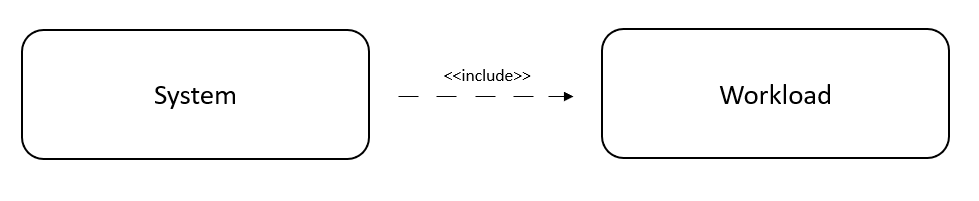
\includegraphics[scale=0.5]{../figures/libraryOverview/libraryOverview.png}
	\caption{Library's components}
\end{figure}
\newpage
\section{Workload}
This part of the library is mainly a C++ class, that lets the user create a specific workload.
\begin{figure}[!htb]
	\centering
	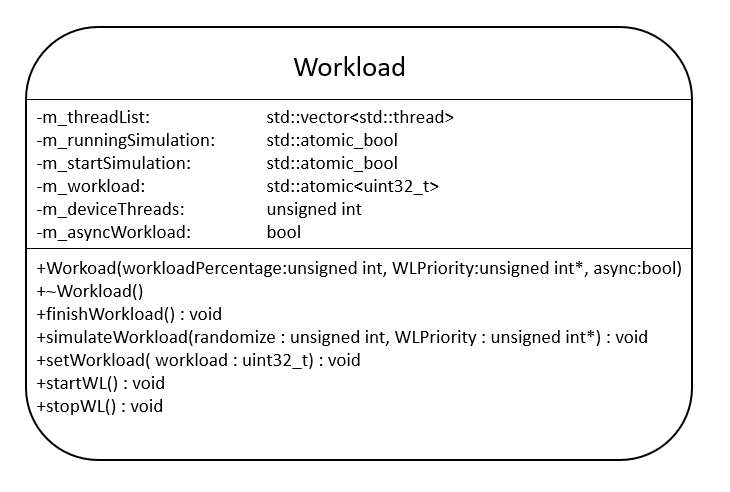
\includegraphics[width=0.7\textwidth]{../figures/libraryOverview/workload.png}
	\caption{Workload class UML}
\end{figure}
\subsection{Attributes}
The class has six private Attributes:
\begin{enumerate}
	\item \texttt{threadList}: is a list of type \textit{std::vector}, that holds the current number of working threads after their initialization
	\item \texttt{runningSimulation}: is a flag that tells the user the status of his working threads. This will be set to true once at least one thread in \textit{threadList} has started executing a routine
	\item \texttt{startSimulation}: is a switch that starts a simulation function (in our case \textit{simulateWorkload()}). This is in order to synchronize threads and start them as simultaneously as possible
	\item \texttt{workload}: hold the current workload set by the user. This is meant for future implementations in order to let the user change workloads dynamically at runtime
	\item \texttt{deviceThreads}: is the number of threads the current machine can handle at the same time. This depends on the processor that the executable is running on, therefore can differ on different device
	\item \texttt{asyncWorkload}: this is a flag for testing purposes in order to simulate a \dq real\dq{} workload. This will be explained in detail later in this chapter.
\end{enumerate}
The names start with \dq m\_\dq{} in order to tell the programmer that the variable is a member of the class. This makes the code more readable for the programmer and informs him about the variable's purpose at the same time, without the need to check the class's definition.

\subsection{Methods}
The class's methods are:
\begin{enumerate}
	\item \texttt{Workload()}: this is the class's constructor and takes three arguemnts:
	\begin{enumerate}
		\item workloadPercentage: workload percentage set by the user to simulate
		\item WLPriority: this is a pointer to a OS-specific thread's priority. If this is set to \textit{NULL}, all threads will have the same (default) priority
		\item async: lets the user to create a more \dq real\dq{} workload.   
	\end{enumerate}
	The first thing the constructor checks when a new object is created is the validity of the passed workload, which cannot be higher than 100 or lower than zero. Next it sets the \textit{runningSimulation} and \textit{startSimulation} attributes to false for a synchronized start. Afterwards it measures the current workload for ten seconds (the time for the measurement can be set to less or more, but ten seconds is in my opinion a proper chunk of time) in order to warn the user for a possible system overload.
	At last, the workload's given percentage is stored in the attribute \textit{workload}, an output will inform the user about the number of threads that will be created and a loop creates the threads, which will run class's \textit{simulateWorkload()} method.\\
	The created threads are pushed into an \textit{std::vector} using \textit{emplace\_back()}. I opted for this method instead of \textit{push\_back()}, because the compiler doesn't have to create the thread, store it temporarily and push it afterwards, but it uses the \textit{std::move} mechanism, where the object is moved directly after the creation. This way we spare ourselves some extra memory (which is a very important factor, if this is used on an ARM architecture)
	\item \texttt{$\sim$Workload()}: this is the class's deconstructor. It is set to default and should be changed for future development. For the moment, I used the \textit{defaul} keyword, but (at some point) the purpose of the destructor should be the object's clean up. For example the joining of the threads in the \textit{threadList} attribute. 
	\item \texttt{finishWorkload()}: this function iterates through the class's thread list, checks if these are joinable (in case some user used detach for some reason) and joins them. In case a thread cannot be joined the \textit{TID} will be printed to the console
	\item \texttt{simulateWorkload()}: this takes two arguments
	\begin{enumerate}
		\item randomize: this is set the index in the thread's construction loop, but should be changed to something better in the future
		\item WLPriority: is the priority passed in the constructor. If this is not \texttt{NULL}, the given priority will be set
	\end{enumerate}
	First the functions increases the priority of the calling thread to maximum, then it waits for all threads to be created. When that happens the attribute \textit{startSimulation} will be set to true. This way we ensure a finer synchronisation between the threads, because reading from a variable and leaving the loop should take less time than the time gap between the thread's creation. Next, each thread sleeps for a couple of milliseconds, if \textit{asyncWorkload} is set so that each thread starts with a small delay in order for the library's workload to be above zero at all times. One can imagine the workload as a sinus curve if the flag is set and a square wave function otherwise (as seen in Figure \ref*{workloadTimeDiagram}).
	\begin{figure*}[!htb]
		\centering
		\subfigure[\texttt{asyncWorkload} not set]{
			\label{syncWorkloadDiagram}
			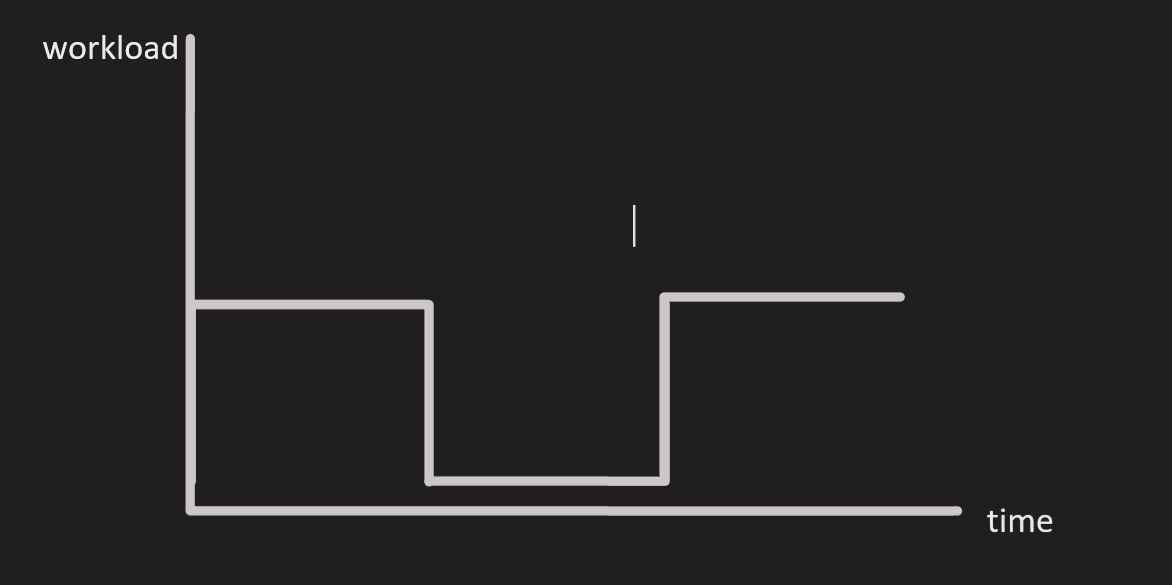
\includegraphics[width=0.7\textwidth]{../figures/libraryOverview/sync_workload.JPG}}
		\subfigure[\texttt{asyncWorkload} set]{
			\label{asyncWorkloadDiagram}
			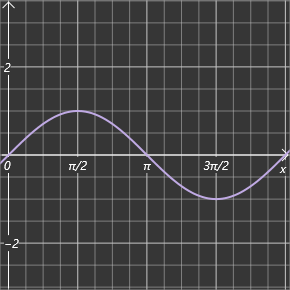
\includegraphics[width=0.4\textwidth]{../figures/libraryOverview/async_workload.png}}
		\caption{Workload Time Diagrams} 
		\label{workloadTimeDiagram}
	\end{figure*}
	Afterwards the actual workload loop will start. I decided to recalculate the sleep time based on the current workload here, in order to support future dynamically changing workload for the simulation. The frequency of the workload is hard coded to ($\frac{2*workload}{100}$)Hz,because a cycle of working and sleeping for a thread is half a second and the system measures the workload once a second so this highly depends on how often the library's system component makes its time measurements.	
	\item \texttt{setWorkload()}: this method's concept is to let the user dynamically change the thread's priority 
	\item \texttt{startWL()}: checks if all threads that needed to be created were saved in the thread list. If this is the case it sets \textit{simulationStart} and \textit{runningSimulation} to true
	\item \texttt{stopWL()}: sets \textit{runningSimulation} to false. It makes sense to call this method before \textit{finishWorkload()}, in order to properly stop all workload threads
\end{enumerate}\newpage
\section{System}
This part of the library mainly contains methods to modify a thread's or process priority, the number of CPUs the process can run on (mentioned in the cpu's affinity section \ref{ssec:cpu_affinity})and the scheduler's policy (mentioned in the operating system's scheduling policies \ref{ssec:sched_policies}).
\begin{figure}[!htb]
	\centering
	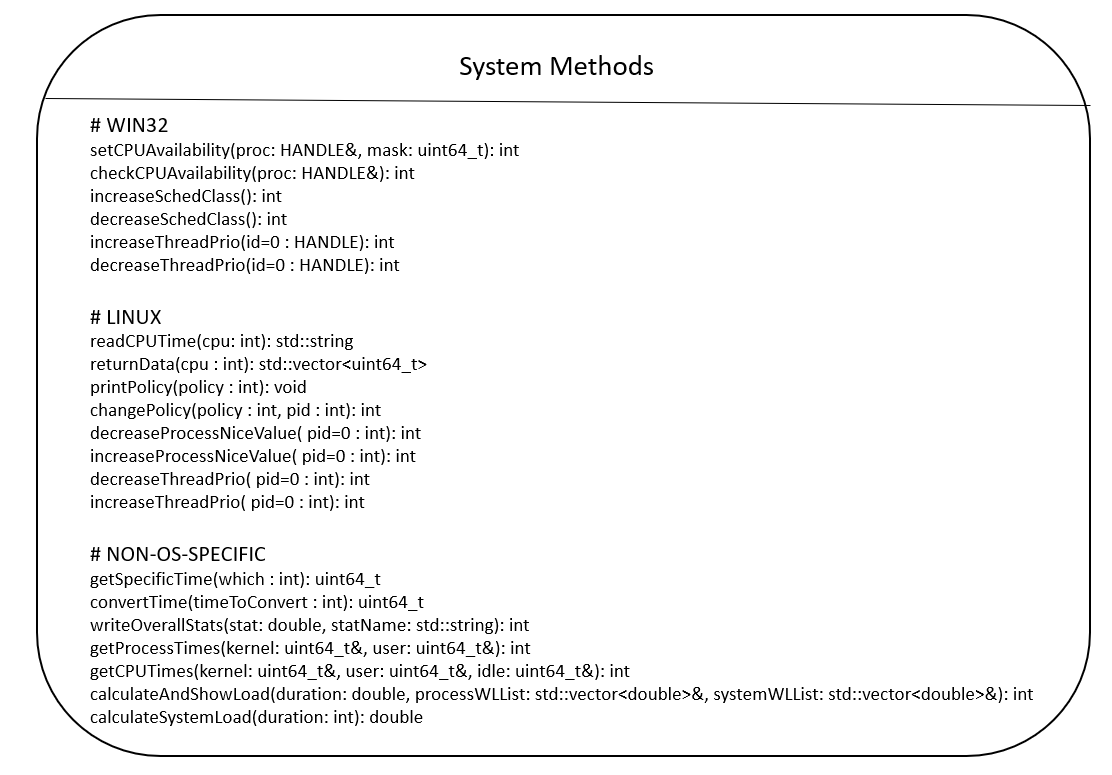
\includegraphics[width=0.7\textwidth]{../figures/libraryOverview/system_methods.png}
	\caption{System Methods}
\end{figure}
\subsection{Defines}
\begin{enumerate}
	\item \texttt{STR\_ERR}: macro returned by a function if it failed
	\item \texttt{IDLE\_TIME}: macro that represents idle time of the system
	\item \texttt{USER\_TIME}: macro that represents user time of the system
	\item \texttt{KERNEL\_TIME}: macro that represents kernel time of the system
	\item \texttt{schedPrioList}: vector containing scheduler classes for a WINDOWS machine in ascending order(mentioned in \ref*{winPrioClass})
	\item \texttt{threadPrioList}: vector containing thread priorities for a WINDOWS machine in ascending order(see \ref*{winPrioClass})
	\item \texttt{sched\_attr}: struct containing thread's attributes for a LINUX machine\cite{linux-man-set/getattribute}
\end{enumerate}
\subsection{Methods}
\label{system-methods}
\begin{enumerate}
	\item Windows:
	\begin{enumerate}
		\item \texttt{mergeFILETIME()}: takes a FILETIME structure as argument, merges the two 32-Bits attributes of the struct into a uint64\_t variable and returns it
		\item \texttt{setCPUAvailability()}:
		\begin{enumerate}
			\item proc: is a windows identification struct for processes of type \texttt{HANDLE}
			\item mask: a 64-Bit value representing the cpu affinity for most computers out there. Each bit represents a cpu. If a bit is set to 1,that means the process can run on the CPU corresponding to that bit.
		\end{enumerate}
		\item \texttt{increaseSchedClass()}:this method gets the current scheduler class and checks if it is already set to the maximum value allowed. In that case it will not do anything, throw an error and return 1. Otherwise it will get the index of the current class in the \textit{schedPrioList}, increase the index by one and set it accordingly. This allows the user to test its program step by step without knowing the actual values in the list. If the user wants to set a certain value for his thread, he can simply use the \textit{winAPI} functions. If one needs to increment the class to the maximum value possible, one can use a while loop in a catch and try block.
		\item \texttt{decreaseSchedClass()}: does almost the same as \textit{increaseSchedClass()}, but instead of increasing the scheduler class's priority, it decreases it. If one wants to decrease the class's value to the minimum one can use a while loop in a catch and try block.
	\end{enumerate}
	\item Linux/Unix:
	\begin{enumerate}
		\item \texttt{readCPUTime()}: this functions takes an argument of type integer and reads data about the CPU specified by the given number using the function \textit{getline()}. For example if your machine has four CPUs, then passing a one will deliver data from the first CPU, passing a two will deliver data for the second CPU and so on. Passing a zero is also acceptable and will deliver data for the whole system (instead of getting individual segments for each CPU, the delivered segments will contain the sum of all CPUs for that specific segment). The data read comes from the \dq/proc/stat\dq{} file. As described in the manual page, the proc filesystem provides informations about the kernel structure or in other words about all processes on the calling system. The \dq/proc/stat\dq{} file contains statistics about the system.\\
		This component uses only the first line and the lines which begin with the name \textit{cpuN}, where \textit{N} stands for the CPU specified by the argument passed to this function. Each line that contains statistics about the CPU has the following pattern\cite{linux-man-proc}:
		\begin{figure}[!htb]
			\centering
			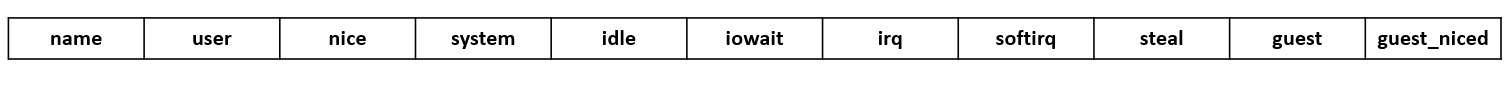
\includegraphics[width=1.1\textwidth]{../figures/libraryOverview/proc_stat.png}
			\caption{Library's components}
		\end{figure}
		The most important statistics for the library are\cite{linux-man-proc}:
		\begin{enumerate}
			\item name: is either cpu or cpuN, where cpu stands for the whole system and cpuN for a cpu specified by N, where N$\in$ [0;max\_number\_of\_CPUs]
			\item user: is the time spent in user mode
			\item nice: is the time spent in user mode with low nice values
			\item system: is the time spent in system mode
			\item idle: is the time spent for idle tasks
		\end{enumerate}
			If the function is successful, it always returns an \texttt{std::string} containing the line specified by the passed argument, else it return the macro \texttt{STR\_ERR}.
		\item \texttt{returnData()}: this function takes an integer as its argument specifying the cpu that we want data from. If the integer is zero, the function returns data from the whole system, one for the first cpu, two for the second cpu and so on. If the given integer is higher than the value returned by \textit{std::thread::hardware\_concurrency()} or lower than zero the function will fail and throw an exception, else the argument will be passed to the \textit{readCPUTime()} method, parse the string returned by it and return the data as an \textit{std::vector} containing \textit{uint64\_t} values.
		\item \texttt{printPolicy()}: this is a utility function that takes an integer as the argument and prints the policy corresponding to it. Possible values are for the arguments are specified in section \ref{ssec:sched_policies}.
		\item \texttt{changePolicy()}: this functions takes two integer as its arguments:
		\begin{enumerate}
			\item policy(int): new policy that should be set
			\item pid(int): the process's \textit{PID}. If this is zero this function will change the policy of the calling process
		\end{enumerate}
		First this function uses system calls, \textit{SYS\_sched\_getattr()} to get the current \textit{sched\_attr struct} specified in the linux man pages and \textit{SYS\_sched\_setattr} to set the new one for the given process specified by the passed arguemnts\cite{linux-man-set/getattribute}.
		\item \texttt{decreaseProcessNiceValue()}: this method takes an integer as its argument specifying the process's PID and is similar to \textit{decreaseSchedClass()}, but instead of checking a local vector list, it uses \textit{getpriority()} with \textit{PRIO\_PROCESS} and \textit{PID} to get the current nice value, saves it temporarily and decreases it by one. Then it uses \textit{setpriority()} to set the new value with the same arguments passed to \textit{getpriority()}. If the nice value reaches 20, the function will throw an exception. The method will fail only if \textit{set/getpriority()} fails.
		\item \texttt{increaseProcessNiceValues()}: this method does the same as its counterpart function mentioned above, but instead of decreasing the value, this method increases it.
	\end{enumerate}
	\item NON-OS-Specific:\\
	NON-OS-Specific functions refrain to methods that either don't depend on any of the OS-Specific libraries such as the UNIX header files and the winAPI or they give the impression of identical behaviour, while in reality each case is manged with a lock-guard. 
	\begin{enumerate}
		\item \texttt{getCPUTimes()}: this function takes the following arguments
		\begin{enumerate}
			\item kernel(uint64\_t reference\footnote{A reference is like a pointer but the variable passed cannot be \textit{NULL}}): kernel time -> time the CPU spent for more \dq privileged\dq{} methods like system calls or interrupts
			\item user(uint64\_t reference): user time -> this refers to any other methods for example a simple loop written by the user
			\item idle(uint64\_t reference): idle time -> this time shows how long the system has been idle 
		\end{enumerate}
		This function gets the three times specified by the arguments and writes them in the passed references for further usage.\\
		On Linux it uses the \textit{returnData()} method with zero as its argument and it saves the first four entries of the returned vector. The zeroth and first entry sum up the user time, the second is the kernel time and the third is the idle time.\\
		On Windows it first creates three FILETIME variables and uses \textit{GetSystemTimes()} to get the three specified times. If \textit{GetSystemTimes()} fails, an exception will be thrown and the function will return one, otherwise it will call \textit{mergeFILETIME()} (because a FILETIME variable is a struct that contains two 32-bit attributes and one needs to concatenate the lower bits to the upper bits to get the real time as a 64-bit variable).
		\item \texttt{getProcessTimes()}: this function takes two uint64\_t references as its arguments and writes the user and kernel times in them. The methods used to get these times do not deliver the idle time (logically thinking there is no user case when this might be important).\\
		On Linux the function calls the \textit{times()} method specified in the \textit{<sys/times.h>} header file. This writes the required times of the calling process in two attributes of type \textit{clock\_t} called \textit{tms\_utime} and \textit{tms\_stime} which belong to a  data type called \textit{struct tms} (this also contains the kernel and user time of any process children created by the current process, but these are irrelevant for this implementation as I use threads instead of processes).\\
		On Windows it uses \textit{GetProcessTimes()} to get the times similar to \textit{getCPUTimes()} and uses \textit{GetCurrentProcess()} to specify the current process. \textit{GetProcessTimes()} also delivers the creation and exit time, however these are irrelevant for this implementation. If \textit{GetProcessTimes()} fails the function will throw an exception and will return one.
		\item \texttt{convertTime()}: this is a utility method and takes a uint64\_t as its argument representing the time. \\
		On Linux \textit{sysconf(\_SC\_CLK\_TCK)} is called, which returns the system's clock ticks per second value. If this fails, an exception is thrown and the functions returns minus one, otherwise it return the seeked time in milliseconds.\\
		On Windows it returns the given argument multiplied by 0.1, which also represents the time in milliseconds.
		\item \texttt{getSpecificCPUTime()}: the method is more utility based and similar to \textit{getCPUTimes()}, but instead of writing its times into the passed arguments, it returns only one time described by the given parameter. Its type is an integer and describes which CPU time should be returned as a uint64\_t value. Possible arguments are \textit{IDLE\_TIME}, \textit{USER\_TIME} and \textit{KERNEL\_TIME}, which are defined in \textit{system/system.hpp} (also mentioned above in the DEFINES section) file and extend to zero, one and two respectively.
		\item \texttt{increase-/decreaseThreadPrio()}: this is similar to \textit{increase-/decreaseProcessNiceValue()} or \textit{increase-/decreaseSchedClass()}.\\
		On Linux the method takes an integer as parameter called \textit{id}, which it gets the current TID's priority, if \textit{id} is zero (which is set by default) or the priority specified by \textit{id} with the help of \textit{sched\_getsched()}. Afterwards it initializes a \textit{sched\_attr} struct, increases/decreases the priority (throws an error if the maximal/minimal priority is reached) and sets the priority through a system call\footnote{Using the system call is preferred, because it supports future development of the function for tempering with more thread's attributes and not only the their priority}. \\
		On Windows it does the same. The only difference is in the parameter and the functions called to get and set the thread's priority. Here the \textit{GetThreadPriority()} and \textit{SetThreadPriority()} are used which expects a HANDLE type as their arguments. That's why we also pass a HANDLE to this function instead on an integer as TID.    
		\item \texttt{calculateSystemLoad()}: the function calculates and returns the system's current workload as a double value\footnote{This is mainly used in the workload class to tell the user the system's current workload and not overload the system}. It takes an integer as its arguments, which specifies the duration of the check.
		On Linux it adds the kernel time to the user time, divides it to the addition of kernel, idle and system time and multiplies the result with 100 to get a workload as a percentage. 
		\begin{equation}
		workload =  \frac{\mathrm{t}_{user}+\mathrm{t}_{kernel}}{\mathrm{t}_{user}+\mathrm{t}_{kernel}+\mathrm{t}_{idle}}*100
		\end{equation}\\
		On Windows however kernel time also contains the idle time of the system (as specified in the winAPI documentation), so in order to get a meaningful and correct result we have to subtract idle time from kernel time.
		\begin{equation}
		workload =  \frac{\mathrm{t}_{kernel}-\mathrm{t}_{idle}+\mathrm{t}_{user}}{\mathrm{t}_{user}+\mathrm{t}_{kernel}}*100
		\end{equation}\\
		\item \texttt{calculateAndShowLoad()}: this functions takes three parameters:
		\begin{enumerate}
			\item duration: the duration of the check while the load simulation is active
			\item processWLList: a \textit{std::vector} that contains entries with the process's workload in one seconds intervals. So the number of entries is also defined by the duration of the check
			\item systenWLList: also a \textit{std::vector}, which contains the system's workloads during the check. It size also depends on the duration of the check 
		\end{enumerate}
		It also calculates the system's and process's workloads using the previous mentioned method. But instead of just printing it to the screen it saves the values into lists (\textit{std::vectors}) used later for writing logging files. Before terminating itself, it also determines the time which the system was not idle using the \textit{convertTime()} and \textit{getSpecficCPUTime()}
		\item \texttt{writeOverallStats()}: this operations takes two arguments:\\
		1) \textit{stat}, which represents the number of the statistic that will be written to the log file\\
		2) \textit{statName}, a string representing the name of the stat\\
		After calling this functions, it will try to create and open a \textit{comma separated file}(CSV) named \dq overall\_stats.csv\dq{}. If this fails an exception will be thrown and the function returns -1. Otherwise it will write the given stat with the given name string passed by \textit{statName} and close the file.
		\item \texttt{wirteRuntimeStats()}: similar to the latter, this functions writes all statistics given by its first argument with the name passed into the second argument to a CSV file. If the CSV file could be successfully created and opened, it will write the statistics and close if afterwards. Otherwise the method will throw an exception and return -1.
	\end{enumerate}
\end{enumerate}
\section{Build System - CMAKE}
As described in \ref{objective} the goal of this thesis is to create methods supporting the two big operating systems in the industry: Linux and Windows. In order to do that, the library comes with additional support for projects that use CMake for their build system. When calling the \textit{cmake} command on the main \textit{CMakeLists.txt}, the system will generate different files depending on the calling OS. When called on Linux, it will generate \textit{Make} files that can be used with the make mechanism that comes with most (almost all) \textit{UNIX} distributions to build the files specified in \textit{CMakeLists.txt} of each directory. When called on Windows, the program will directly create the binaries specified in the main CMakeFileLists.txt. If the Windows machine has \textit{Visual Studio Studio} installed, CMake will also create a solution of the project that can be used for further development and debugging.\\
We can use the CMake syntax to either link the components to the library statically or dynamically\footnote{Static Library means that the linked libraries will be part of the executable, while the code from a Dynamically Linked Library will be linked at runtime, thus resulting in a much smaller sized executable. A good hint for the user when trying to link this library}. 
\subsection{Implementation}
\begin{wrapfigure}{1}{0.5\textwidth}
	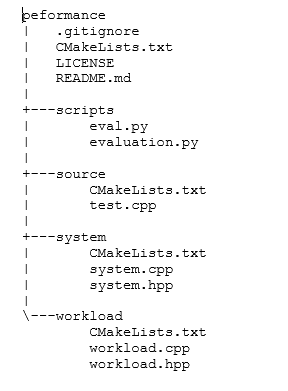
\includegraphics[width=.8\linewidth]{../figures/libraryOverview/performance_tree.png}
	\caption{Library's directory tree}
	\label{directory_tree}
\end{wrapfigure}
As already mentioned, when using \textit{CMake} each directory needs a \textit{CMakeLists.txt}. The main file is the most important file, because it sets the requirements for the whole project.\\
The first requirement for this project is the minimum cmake version, which is set from 3.12 to 3.21. Then a failing criteria is set, for the user to know, that the library doesn't support older versions than 3.12. This way the user does not have to have the newest versions, but we should also make them update their CMake program if it's too old. Afterwards some CMake standard variables are set to make the user have at least C++17 enabled. These settings are written for two main reasons: \\
First, the library uses newer elements for its components, therefore older versions won't be compatible and so errors will occur.\\
Second, the library should encourage the users to start implementing modern and up-to-date standards and companies should opt for a the newer tools as they often have more to offer(in my opinion C++17 cannot be even seen as a new standard anymore, considering that at the time of writing the newest (with a final version) Cpp Standard is C++20 and with C++23 already in development with full integration for the GCC compiler).\\
After that the library prints a message to tell the user what operating system was recognized by CMake and then we define the name of the project, the version, description and its programming language.\\
Finally we tell CMake which directories contain the code for our project by adding them to the include search path and linking the targets that are defined in those directories to the main executable target created in the \textit{CMakeLists.txt} that can be found in the source subdirectory.\\ 
Unfortunately, during the development phase, linking the components dynamically lead to errors and because of the lack of time, the components were linked statically.\\
Each component has its own \textit{CMakeLists.txt}. The workload components first creates a static library/target with the appropriate header and source files, sets the \\ \textit{THREADS\_PREFER\_PTHREAD\_FLAG} to ON and searches for the \textit{pthread} library. If this is found the compilation continues, otherwise an error will be raised, because of the component's thread implementation. Afterwards it includes the system's component directory to its search path and links against it and against the pthread library. At the end, it specifies that the compiled binary (windows .lib-file and Linux .o-file\footnote{If the library was dynamically linked on windows we would get a .dll-file and on Linux a .so-file}) needs to be created in the binary directory specified by \textit{CMake} in a subdirectory called \dq lib\dq{}.\\
The system component has a much simpler \textit{CMakeLists.txt}. It only creates the target with the specific header and source files and specifies where the compiled library will be created, which is the same directory as for the workload component.\\
A detailed directory tree of the library can be seen in figure \ref{directory_tree}
%\begin{figure}[!htbp]
%	\centering
%	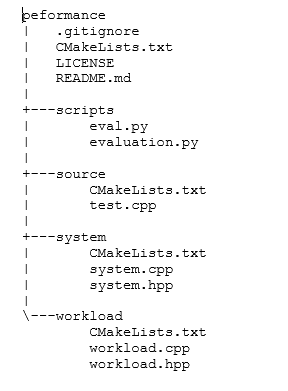
\includegraphics[scale=0.3]{../figures/libraryOverview/performance_tree.png}
%	\caption{Library's directory tree}
%	\label{directory_tree}
%\end{figure}
